\documentclass[10pt,letterpaper]{article}
\usepackage[top=1in,bottom=1in,left=1in,right=1in]{geometry}
\usepackage{datetime}
\usepackage{natbib}      % http://merkel.zoneo.net/Latex/natbib.php
\usepackage{palatino}
\usepackage{verbatim}
\usepackage[normalem]{ulem}
\bibpunct{(}{)}{;}{a}{,}{,}

\usepackage{array}

\usepackage{chngpage}
\usepackage{stmaryrd}
\usepackage{amssymb}
\usepackage{amsmath}
\usepackage{graphicx}
\usepackage{lscape}
\usepackage{subfigure}
\usepackage[usenames,dvipsnames]{color}
\definecolor{myblue}{rgb}{0,0.1,0.6}
\definecolor{mygreen}{rgb}{0,0.3,0.1}
\usepackage[colorlinks=true,linkcolor=black,citecolor=mygreen,urlcolor=myblue]{hyperref}

\newcommand{\bocomment}[1]{\textcolor{Bittersweet}{BO says: #1}}

\newcommand{\ignore}[1]{}
\newcommand{\transpose}{^\mathsf{T}}
\newcommand{\inner}[1]{\langle #1 \rangle} 
\newcommand{\smallsec}[1]{\noindent \textbf{#1\ }}
\newcommand{\cmd}[1] {{\color{blue}\texttt{#1}}}

\newcommand{\solution}[1]{{\color{myblue} \emph{[Solution:} 
#1 

\emph{End solution]}}}
\newcommand{\solutionnote}[1]{{\color{myblue} \emph{[Note:}

#1 

\emph{End note]}}}
\newcommand{\points}[1]{{\color{mygreen}\emph{[#1]\ \ }}}

\newcommand{\aone}{\diamondsuit}
\newcommand{\atwo}{\heartsuit}
\newcommand{\bone}{\triangle}
\newcommand{\btwo}{\Box}
\newcommand{\myand}{\ \land\ }
\newcommand{\myor}{\ \lor\ }
\newcommand{\mynot}{\lnot}

\title{
  \textbf{Mini-project 2} \\
  \Large{CMPSCI 670, Fall 2016, UMass Amherst} \\
  \Large{Due:  October 14, 5:00 PM } \\
  \Large{Instructor: Subhransu Maji} \\
  \Large{TA: Tsung-Yu Lin}
}

\settimeformat{ampmtime}
\date{}
\begin{document}
\maketitle

\renewcommand\thesubsection{\thesection.\alph{subsection}}


\section*{Guidelines}

\paragraph{Submission.} Submit a \emph{single pdf document} via moodle that includes your solutions, figures and printouts of code. For readability you may attach the code printouts at the end of the solutions. You could have 24 hours late submission with a 50\% mark down. Late submission beyond 24 hours will not be given \emph{any} credits. 

\paragraph{Plagiarism.} We might reuse problem set questions from previous years, covered by papers and webpages, we expect the students not to copy, refer to, or look at the solutions in preparing their answers. We expect students to want to learn and not google for answers. 

\paragraph{Collaboration.} The homework must be done individually, except where otherwise noted in the assignments. 'Individually' means each student must hand in their own answers, and each student must write their own code in the programming part of the assignment. It is acceptable, however, for students to collaborate in figuring out answers and helping each other solve the problems. We will be assuming that you will be taking the responsibility to make sure you personally understand the solution to any work arising from such a collaboration.

\paragraph{Using other programming languages.} All of the starter code is in Matlab which is what we expect you to use. You are free to use other languages such as Octave or Python with the caveat that we won't be able to answer or debug non Matlab questions.



\newpage

\section{Hybrid image [20 points]}
A hybrid image is a combination of a low-pass filtered (i.e. blurry) image and a high-pass filtered (i.e. sharp) image. Recall that one can obtain a sharp image by subtracting the blurry version of an image from itself. Mathematically this can be written as $I = blurry(I) + sharp(I)$. Thus a hybrid image of $I_1$ and $I_2$ can be obtained as: 
\begin{equation}\label{eq:hybrid}
	I_{hybrid} = blurry(I_1, \sigma_1) + sharp(I_2, \sigma_2) = I_1 * g(\sigma_1) + I_2 - I_2*g(\sigma_2).
\end{equation}

Here, $g(\sigma_1)$ and $g(\sigma_2)$ are Gaussian filters with standard deviations $\sigma_1$ and $\sigma_2$ and * denotes the filtering operator. Figure~\ref{fig:blur} shows the result of filtering with Gaussians of two different $\sigma$ values.


\begin{figure}[h]
\begin{tabular}{cccc}
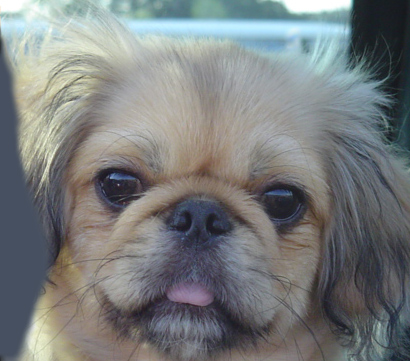
\includegraphics[width=0.23\linewidth]{./output/dog.jpg} &
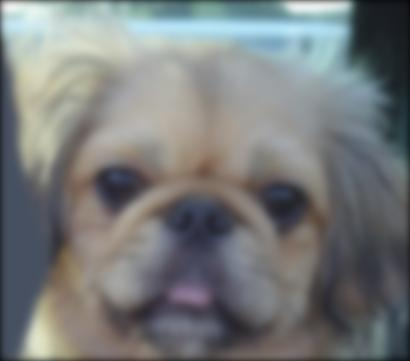
\includegraphics[width=0.23\linewidth]{./output/dog-blurry-4.jpg} & 
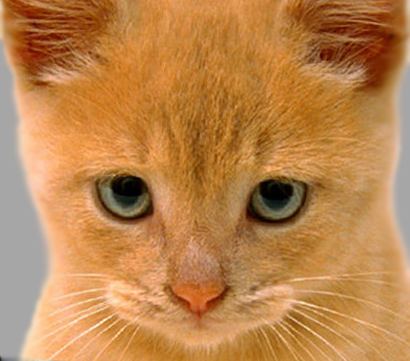
\includegraphics[width=0.23\linewidth]{./output/cat.jpg} &
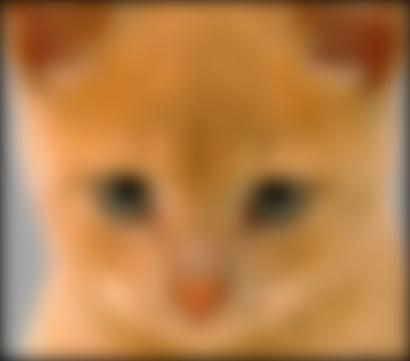
\includegraphics[width=0.23\linewidth]{./output/cat-blurry-10.jpg}\\
dog image & $\sigma=4$ & cat image & $\sigma=10$ \\
\end{tabular}
\caption{\label{fig:blur} Effect of filtering with a Gaussian. The bigger the sigma the more blurry it is.}
\end{figure}

Implement the function $\cmd{hybridImage(im1, im2, sigma1, sigma2)}$ that computes the hybrid image using Equation~\ref{eq:hybrid}. Use your code to generate at least one example of a hybrid image (see examples here \url{http://cvcl.mit.edu/hybrid_gallery/gallery.html}). You will have to tune the $\cmd{sigma1}$ and $\cmd{sigma2}$ to make it work on specific images. In order to visualize the hybrid image it is sometimes useful to show multiple copies of the image at different resolutions. You can use the function $\cmd{vis\_hybrid\_image.m}$ included in \cmd{p2\_code.zip} which can be used to create such a figure. Include the code, the two source images, the hybrid image displayed in the format below, as well as the parameters that worked for you. \emph{The three most creative submissions will be given a prize.}

\begin{figure}[h]
\centering
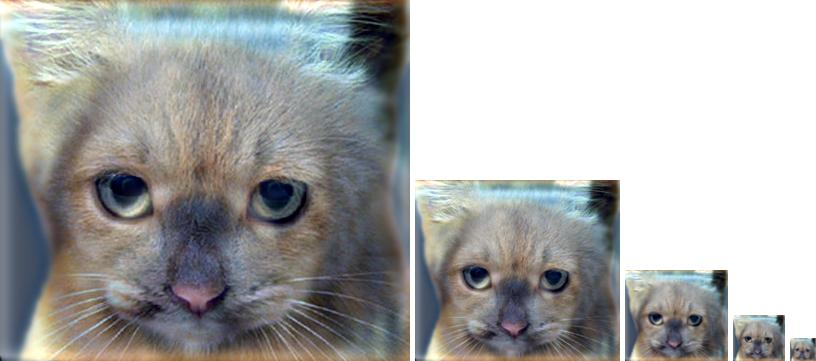
\includegraphics[width=0.85\linewidth]{./output/hybrid-4-10.jpg}
\caption{Hybid image of the dog and cat. The large image looks like the cat while the small image looks like the dog. The image was created with $\sigma_1 = 4$ and $\sigma_2 = 10$.}
\end{figure}


\newpage

\section{Photometric stereo [50 points]}


In this part you will implement a basic shape from shading algorithm as described in Lecture 5. This is also described in shape from shading section (Sec 2.2) in Forsyth and Ponce book (\href{http://www.sci.utah.edu/~gerig/CS6320-S2012/Materials/Forsyth-Ponce-SfS.pdf}{pdf link} for this section). The input to the algorithm is a set of photographs taken in known lighting directions and the output of the algorithm is the albedo (paint), normal direction, and the height map (Figure~\ref{fig:photometric-stereo}).


If you haven't done so already, download the \cmd{p2\_code.zip} and \cmd{p2\_data.zip} files from moodle. The data directory consists of 64 images each of four subjects from the Yale Face database. The light source directions are encoded in the file names. 


\begin{figure}[h]
\centering
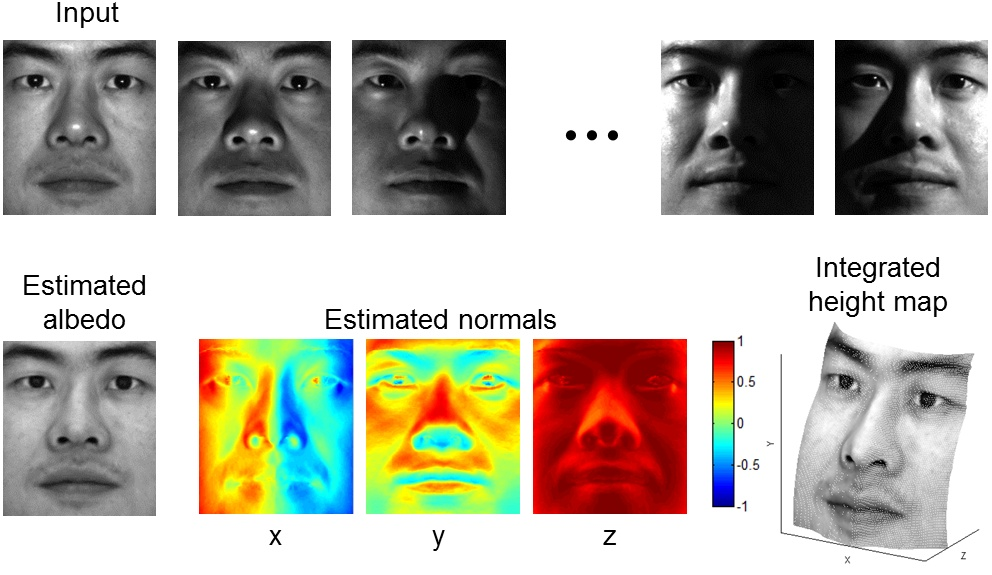
\includegraphics[width=0.85\linewidth]{./fig/shape_from_shading.jpg} \\
\caption{\label{fig:photometric-stereo} Top row: Input images. Bottom row: Estimated albedo, normals, and depth map}
\end{figure}


Below is an outline of the steps you need to implement the functions. The entry code for this part is \cmd{evalCode.m}. You will add code to files \cmd{prepareData.m}, \cmd{photometricStereo.m} and \cmd{getSurface.m} as described below. The remaining files are for processing the input data and displaying the output.

\begin{enumerate}

\item \textbf{Read images and light sources.} For each subject (sub-directory in the \cmd{data} folder), read in the images and light source directions. This is accomplished by the function \cmd{loadFaceImages.m} (which, in turn, calls \cmd{getpgmraw.m} to read the PGM files). The function \cmd{loadFaceImages()} returns the images for the 64 light source directions, an ambient image (i.e., image taken with all the light sources turned off), and the light directions for each image.

\item \textbf{[5 points] Preprocess the data.} We need the images under the illumination of only the point light source. Fortunately, due to linearity of light we can do this by subtracting the ambient image from all the images. Also, set any negative values to zero and rescale the resulting intensities to between 0 and 1 by dividing by 255. Implement this in the \cmd{prepareData.m} file.


\item \textbf{[20 points] Estimate the albedo and  normals.} Implement the function in  \cmd{photometricStereo.m} which takes as input the stack of images and the matrix of the light source directions, and returns an albedo image and normal directions. The normal directions should be encoded as a three dimensional array of size $h \times w \times 3$ where the third dimension corresponds to the x-, y-, and z-components of the normal. To solve for the albedo and the normals, you will need to set up a linear system as shown in slide 80 of Lecture 5.

To get the least-squares solution of a linear system, use MATLAB's backslash operator. That is, the solution to \cmd{Ax = b} is given by \cmd{x = A\textbackslash b}. If you directly implement the formulation of slide 80 of the lecture, you will have to loop over every image pixel and separately solve a linear system in each iteration. There is a way to get all the solutions at once by stacking the unknown $g$ vectors for every pixel into a $3 \times n$ pixels matrix and getting all the solutions with a single application of the backslash operator.
You will most likely need to reshape your data in various ways before and after solving the linear system. Useful MATLAB functions for this include \cmd{reshape} and \cmd{cat}.
You may also need to use element-wise operations. For example, for two equal-size matrices $\mathbf{X}$ and $\mathbf{Y}$, $\mathbf{X}$.* $\mathbf{Y}$ multiplies corresponding elements, and $\mathbf{X}.^\wedge 2$ squares every element. As before, \cmd{bsxfun()} can also be a very useful function here.

\item \textbf{[20 points] Compute the surface height map by integration.} The method is shown in slide 83 of Lecture 5, except that instead of continuous integration of the partial derivatives over a path, you will simply be summing their discrete values. Your code implementing the integration should go in the \cmd{getSurface.m} file. As stated in the slide, to get the best results, you should compute integrals over multiple paths and average the results. You should implement the following variants of integration: 
\begin{itemize}
\item Integrating first the rows, then the columns. That is, your path first goes along the same row as the pixel along the top, and then goes vertically down to the pixel. It is possible to implement this without nested loops using the \cmd{cumsum()} function.
\item Integrating first along the columns, then the rows.
\item Average of the first two options.
\item Average of multiple random paths. For this, it is fine to use nested loops. You should determine the number of paths experimentally.
\end{itemize}

\item Display the results using \cmd{displayOutput} and \cmd{plotSurfaceNormals} functions.

\end{enumerate}

\textbf{Hint:} You can start by setting the \cmd{subjectName='debug'} which creates images from a toy scene with known geometry and albedo. You can debug your code against this before you try the faces.

\subsection{What to submit}
To get full credit for this part you have to
\begin{itemize}
\item Include your implementation of \cmd{prepareData.m}, \cmd{photmetricStereo.m}, and \cmd{getSurface.m}. Also, include the visualization of albedo image, estimated surface normals, and recovered surface of four subjects. It is sufficient to simply show the output of your best method. For the 3D screenshots, be sure to choose a viewpoint that makes the structure as clear as possible (and/or feel free to include screenshots from multiple viewpoints)
\item \textbf{[5 points]} Discuss the differences between the different integration methods you have implemented. Specifically, you should choose one subject, display the outputs for all of a-d (be sure to choose viewpoints that make the differences especially visible), and discuss which method produces the best results and why. Also, discuss how the Yale Face data violate the assumptions of the shape-from-shading method covered in the slides.
\end{itemize}

\newpage
\section{Extensions}

On this assignment, there are not too many opportunities for "easy" extra credit. This said, here are some ideas for exploration:
\begin{itemize}
\item Generate synthetic input data using a 3D model and a graphics renderer and run your method on this data. Do you get better results than on the face data? How close do you get to the ground truth (i.e., the true surface shape and albedo)?
\item Investigate more advanced methods for shape from shading or surface reconstruction from normal fields.
\item Try to detect and/or correct misalignment problems in the initial images and see if you can improve the solution.
\item Using your initial solution, try to detect areas of the original images that do not meet the assumptions of the method (shadows, specularities, etc.). Then try to recompute the solution without that data and see if you can improve the quality of the solution.
\end{itemize}
If you complete any work for extra credit, be sure to clearly mark that work in your report, explain it and include the code.



\end{document}
